\documentclass{article}
\usepackage{caption}
\usepackage{cancel}
\usepackage{tikz}
\usepackage[fontsize=16pt]{fontsize}

\author{Mike McLennan}
\date{}
\title{Subtraction\\
\vspace{28pt}
\begin{normalsize}Applied Scholastics, Ferndale WA \end{normalsize}}

\begin{document}
\maketitle
\pagebreak
\tableofcontents
\pagebreak

\section{Subtraction}
Subtract is a Latin word meaning to pull away. The Sub- means under or away, and the -tract means to pull, as in a tractor.

To subtract a number is to take that value away from another number.\\

Minus is a Latin word meaning less.

The minus symbol $-$ is used in writing subtraction. It comes from an m with a line over it, $\bar{\textrm{m}}$, which was once short for the word minus.\\

The number being subtracted is called the subtrahend.\\

The number it is being subtracted from is called the minuend.\\

The result of subtracting one number from another is called the difference.\\

$$8 - 3 = 5$$


minuend - subtrahend = difference

\newpage

Subtraction is the opposite of Addition. If you know your addition table for single-digit numbers then you also know how to subtract them.

\begin{center}
$5 + 3 = 8$, so $8 - 3 = 5$
\end{center}

\vspace{32pt}
You can use a number line to show what is happening. Moving to the right on the line represents adding, and moving to the left on the line represents subtracting. Here is $2+3=5$:\\

\begin{center}
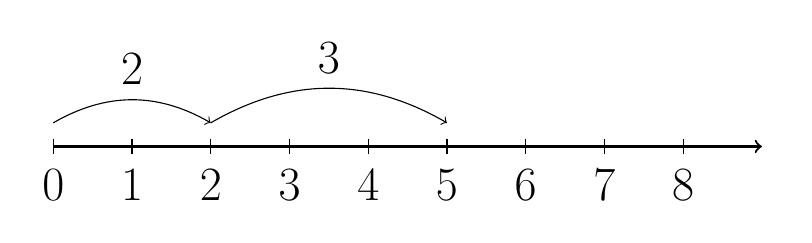
\begin{tikzpicture}
\draw[thick, ->] (0,0) -- (9,0) node[below] {$\ $};
\foreach \n in {0,1,2,3,4,5,6,7,8} {\draw (\n,0.1) -- (\n,-0.1) node[below] {$\n$};}
\draw[->, bend left=30] (0,0.3) to node[above] {$2$} (2,0.3);
\draw[->, bend left=30] (2,0.3) to node[above] {$3$} (5,0.3);
\end{tikzpicture}
\end{center}

And here is $5-3=2$:

\begin{center}
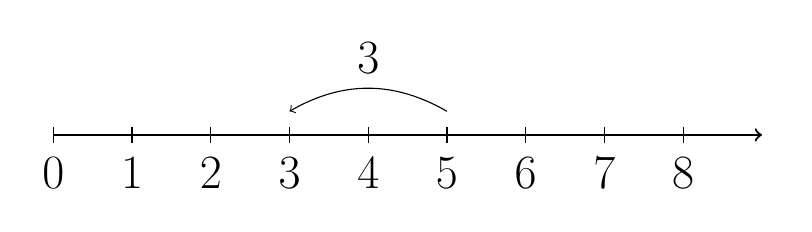
\begin{tikzpicture}
\draw[thick, ->] (0,0) -- (9,0) node[below] {$\ $};
\foreach \n in {0,1,2,3,4,5,6,7,8} {\draw (\n,0.1) -- (\n,-0.1) node[below] {$\n$};}
\draw[<-, bend left=30] (3,0.3) to node[above] {$3$} (5,0.3);
\end{tikzpicture}
\end{center}

The minuend has to be larger than the subtrahend or the difference will be less than zero, which is another subject.

\newpage

\section{Subtraction in Columns}
Subtracting multi-digit numbers is done by arranging the numbers into columns aligned at the decimal point. Each column of digits is subtracted separately to get a difference.

$72 - 21$ can be solved by $7 - 2 = 5$ and $2 - 1 = 1$ resulting in a difference of 51:

\begin{center}
\begin{tabular}{c@{\,}c@{\,}c@{\,}}
 & &\text{ minuend}\\
-& &\text{ subtrahend}\\
\hline
=& &\text{ difference}\\
\hline
\hline
\end{tabular}
\end{center}

\begin{center}
\begin{tabular}{c@{\,}c@{\,}c@{\,}}
 &7&2\\
-&2&1\\
\hline
=&5&1\\
\hline
\hline
\end{tabular}
\end{center}

\vspace{14pt}
The difference is separated from the minuend and subtrahend by a single line, and is double underlined to indicate that this is a final answer.\\

Numbers, of any length, can be subtracted in this way, with the units, tens, thousands, and so on all aligned into columns to make the operation clear and simple.\\

\begin{center}
\begin{tabular}{c@{\,}c@{\,}c@{\,}c@{\,}c@{\,}c@{\,}c@{\,}c@{\,}}
  & &1&0&4,&2&1&3\\
 -& & & &3,&1&1&2\\
\hline
= & &1&0&1,&1&0&1\\
\hline
\hline
\end{tabular}\\
\end{center}

\newpage

\section{Borrowing}
In addition in columns we had the situation where a subtotal could be greater than 9 so that the 10s value had to be carried over to the next higher column.

We have the opposite problem in subtracting in columns. Sometimes the subtrahend is greater than the minuend so the difference would be less than 0. It's solved by borrowing from the next highest column.

\begin{center}
\begin{tabular}{c@{\,}c@{\,}c@{\,}c@{\,}c}
& & &^{4}\cancel{5}&^{1}3\\
   - & & &1&5\\
	\hline
	& & &3&8\\
	\hline
	\hline
\end{tabular}
\end{center}

\begin{center}
\begin{tabular}{c@{\,}c@{\,}c@{\,}c@{\,}c}
&^2\cancel{3},&^{13}\cancel{4}&^{14}\cancel{5}&^{1}6\\
   - & &7&8&9\\
	\hline
	&2,&6&6&7\\
	\hline
	\hline
\end{tabular}
\end{center}

As you can see, sometimes borrowing can get into chains of borrowing before the subtraction can be done.

\begin{center}
\begin{tabular}{c@{\,}c@{\,}c@{\,}c@{\,}c}
&^0\cancel{1},&^{9}\cancel{{^{1}0}}&^{9}\cancel{{{^1}0}}&^{1}0\\
   - & &7&8&9\\
	\hline
	&2,&6&6&7\\
	\hline
	\hline
\end{tabular}
\end{center}

\newpage

\section{Adding and Subtracting\\by Equal Adjustment}
Sometimes when adding or subtracting two numbers it is easier to add or subtract a small amount to both number, to make the units digit equal to zero. You don't have to carry or borrow digits this way.\\

For example, $78 + 96$ is the same as $78 + 2 + 96 - 2$. You are just adding two and taking it away again, leaving the sum unchanged. It is easier to add $80 + 94$ than to add $78 + 96$, but they both result in the same sum.\\

In the same way, $96 - 78$ is the same as $96 + 2 - 78 + 2$. The difference remains the same. $98 - 80$ is a much easier problem to solve.

\newpage

\section{Checking Subtraction}

Subtraction can be checked by rearranging the terms to make an addition. If $a-b=c$ then $c+b=a$. There is no need to write out the addition because the digits can be added upward mentally.\\

Casting out 9s and finding digit sums can be done but is not as useful as for addition, where there may be a long list of numbers, because with subtraction you are usually only dealing with two numbers.\\

\begin{center}
\begin{tabular}{c@{\,}c@{\,}c@{\,}c@{\,}c}
& &1&^{4}\cancel{5}&^{1}3\\
   - & & &1&5\\
	\hline
	& &1&3&8\\
	\hline
	\hline
\end{tabular}
\end{center}

If the digit sum of the subtrahend is larger than the digit sum of the minuend, you can either add 9 to the minuend, or you can rearrange the subtraction into an addition.\\

Digits sum for 153 is $1+5+3 = 9 = 0$. Add 9 to make it larger than the subtrahend. The digit sum for 15 is $1 + 5 = 6$. Digit sum for 138 is 3. $9 - 3 = 6$ so the answer is probably correct.\\

\newpage
\

\begin{center}
\linespread{2}\large

Enquiries

\textbf{Applied Scholastics Ferndale}

Principal: Paula McLennan

mobile phone: 0431 683 306

email address: apsferndale@gmail.com

website: apsferndale.webs.com
\end{center}

\end{document}
